\chapter{Evaluation} \label{Evaluation}

\section{Testing}

\subsection{Bound Box downloads vs Individual Field downloads}
Bounding boxes = fast but less accurate data, individual fields = slower but more accurate.

\section{Results}
With the current version of the system complete, it is able to take a shapefile dataset from the \acrshort{DEPA}\cite{Jordbrugsanalyser} and input all fields of a specific type into the database, with field ID's, crop type, CVR number and the geometry polygon used for the API. A workload for the download workers can then be started, to download remote sensing data in a given time range for each field and input it to the database, either using bounding boxes or individual fields. A separate workload for the process workers can then be started, to process different vegetation indices for each field. Separate graph maker functions allow for visual representation of further field analysis.

\subsection{NDVI Field Analysis}
This section focuses on whether an NDVI analysis of a given field with seed potatoes follow the general growth period and standards presented if the domain analysis section \ref{Growth Period}. This will be done on a field growing seed potatoes in 2020 and can be seen on figure \ref{fig:2443NDVIavg}.
\begin{figure}[h]
    \centering
    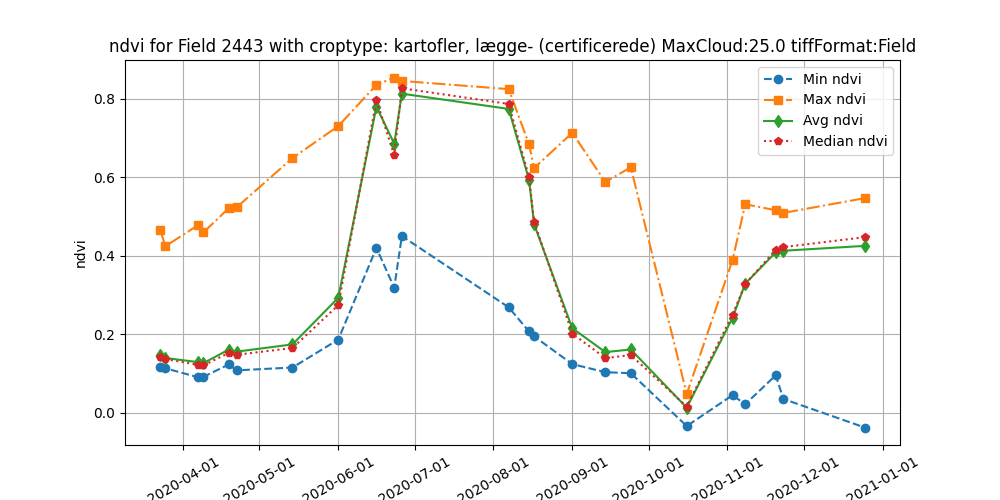
\includegraphics[width=0.75\linewidth]{images//results/Field2443NDVIGraph.png}
    \caption{NDVI readings for Field ID 2443, seed potatoes (25\% max cloud coverage)}
    \label{fig:2443NDVIavg}
\end{figure}

As a preliminary, there are data points missing. Even though the Sentinel-2 satellites circle Denmark every 3-5 day, if the cloud cover is significant enough there is too much noise to give accurate readings for vegetation indices. Because of this, any day with available data where the cloud coverage was over 25\% is excluded.

Aforementioned in the domain analysis, seed potatoes are planted late March throughout April. During the period the field should be rather barren and NDVI values low, in accordance to the figure. The max NDVI readings are higher. Assumably because of stray weeds or perhaps the polygon geometry had some inaccuracies and  included some flora, bushes or trees. Assuming the potatoes were planted mid to late April, the NDVI readings start increasing in the middle of May in accordance to the 2-6 weeks germination period. Throughout June and July an average NDVI reading of just below 0,8 is observed, indicating healthy dense vegetation. This is should be the case, as the canopy of the potato plants has a dense leaf area coverage.

On August 7th the average NDVI value is still saturated just below 0,8. But on the next reading on August 15th, the readings have dropped to just below 0,6. Such a significant drop provokes the assumption of pre-harvest crop desiccant usage. This drop in NDVI value continues throughout August and levels out in the middle to late September. This 20 day significant drop in NDVI value is in accordance with the desiccation time of desiccant Mizuki, as described in section \ref{Pre-harvest desiccation agents}. An assumption can be made on the basis of popularity and desiccation time, that Mizuki was used on or shortly after August 10th.

During this period it is observed that the maximum NDVI value fluctuates a bit and does not have a drop off like the average NDVI. This could be the result of stray weeds taking advantage of newly available sunlight, as the potato canopies wilt. But on the 16th October it drops to near 0 along with the average. It is assumed that harvest happened on or around the 16th, turning over all of the plants, leaving only soil visible. The next available reading is on the 29th of October and the NDVI value increases again, presumably due to weeds and other natural flora beginning to grow on the empty field.

\subsubsection{Heat maps}
These assumptions can be further explored using heat maps during the period of interest, August throughout October. The full set of heat maps over the period can be seen in appendix \ref{EvaluationResults}. 

\begin{figure}[htbp]
  \centering
  \begin{minipage}[b]{0.40\textwidth}
    \centering
    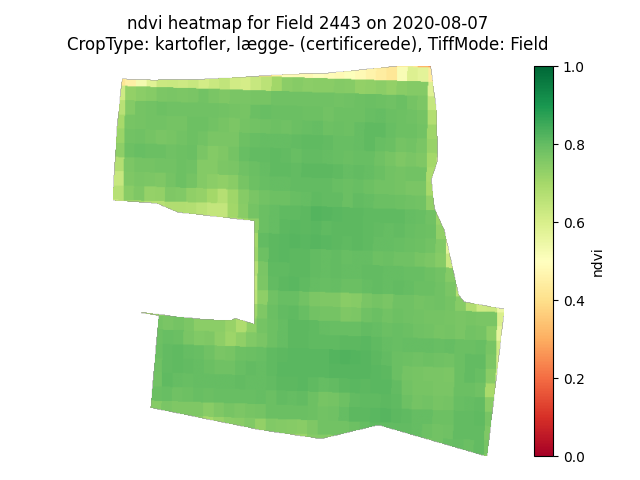
\includegraphics[width=\textwidth]{images/results/HeatmapsNDVI2443/HeatMapndvi_2443_kartofler_lgge-_certificerede_2020-08-07_Field.png}
    \caption{NDVI Heatmap August 7th (25\% max cloud coverage)}
    \label{fig:Heatmap7thAugust}
  \end{minipage}
  \hfill
  \begin{minipage}[b]{0.40\textwidth}
    \centering
    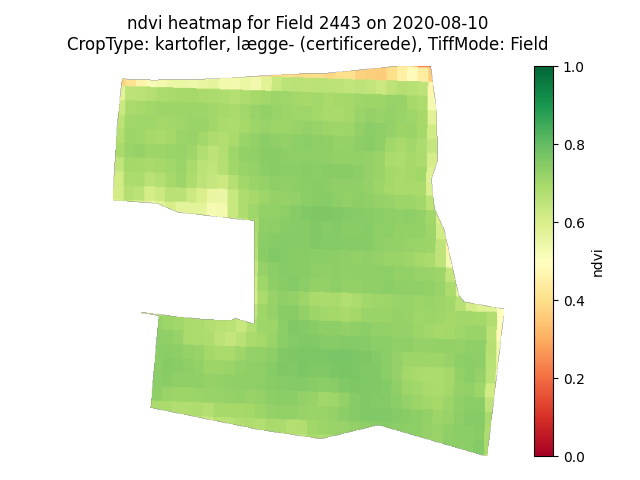
\includegraphics[width=\textwidth]{images/results/HeatmapsNDVI2443/HeatMapndvi_2443_kartofler_lgge-_certificerede_2020-08-10_Field.png}
    \caption{NDVI Heatmap August 10th (25\% max cloud coverage)}
    \label{fig:Heatmap10thAugust}
  \end{minipage}
\end{figure}
The assumed indication of pre-harvest crop desiccant use on August 7th. On figure \ref{fig:Heatmap7thAugust} the field is green and rather saturated. Notably, in the top right of the figure the values are rather low at approximately 0,5. It is assumed that there was not space for another trench to plant potatoes there and that section of the field did not contain any potato plants. Three days later an approximate 0.1 drop in NDVI value can be seen across the field, as seen on figure \ref{fig:Heatmap10thAugust}. On August 15th \ref{fig:Heatmap15thAugust} the average NDVI value is around 0,6. Such a drop in NDVI values is a clear indicator of stressed vegetation. And since it is in the pre-harvest crop desiccation usage period, it is further assumed to be the causation.

\begin{figure}[htbp]
  \centering
  \begin{minipage}[b]{0.40\textwidth}
    \centering
    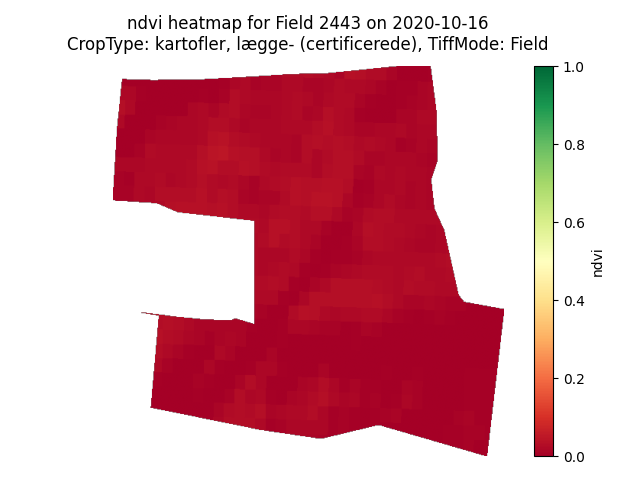
\includegraphics[width=\textwidth]{images/results/HeatmapsNDVI2443/HeatMapndvi_2443_kartofler_lgge-_certificerede_2020-10-16_Field.png}
    \caption{NDVI Heatmap October 16th (25\% max cloud coverage)}
    \label{fig:Heatmap16thOctober}
  \end{minipage}
  \hfill
  \begin{minipage}[b]{0.40\textwidth}
    \centering
    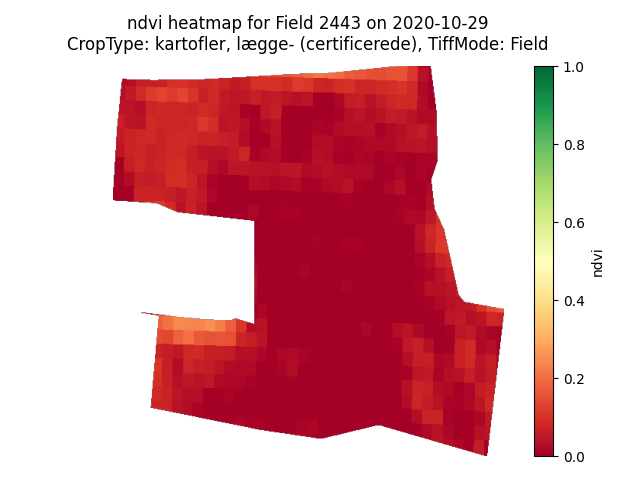
\includegraphics[width=\textwidth]{images/results/HeatmapsNDVI2443/HeatMapndvi_2443_kartofler_lgge-_certificerede_2020-10-29_Field.png}
    \caption{NDVI Heatmap October 29th (25\% max cloud coverage)}
    \label{fig:Heatmap29thOctober}
  \end{minipage}
\end{figure}

It is further solidified that the harvest came on or around October 16th when looking at figure \ref{fig:Heatmap29thOctober}, as the entire field is dark red signifying no vegetative growth on the field. Notably, the top right of the field is also dark red. This indicates that it was not bushes or trees overlapping on the field. Why the NDVI readings in that section were lower on the previous readings (figure \ref{fig:Heatmap7thAugust} and \ref{fig:Heatmap10thAugust}) is unknown. Perhaps potatoes were not planted there due to lack of space in terms of trench spacing. Or maybe that segment of the field was not properly fertilized and the potatoes growing there lacked the proper nutrients, leading to lower chlorophyll levels and in turn, NDVI levels. In correlation with figure \ref{fig:2443NDVIavg}, figure \ref{fig:Heatmap29thOctober} shows minor vegetation starting to sprout after the harvest around October 16th on the next available reading, the October 29th.

\subsection{Other vegetation indices}
In the domain analysis in section \ref{Vegetation indices}, a series of different vegetation indices were analysed, in regards to their ranges, spectral bands and specific use cases they are best suited for. This section analyses the results of other vegetation indices and explores whether they are better suited or can compliment the NDVI index, in the pursuit of detecting pre-harvest crop desiccant overuse.

While CVI is focused on detecting stressed vegetation, it is most commonly used to detect nutrient deficiencies in the soil, which in turn leads to stressed vegetation, in the early to mid growth period. Additionally, it does not have a normalized range and is context based, making it difficult to compare directly with NDVI.

Both EVI and GNDVI show the same story of the growth period of the potatoes as NDVI as seen on figure \ref{fig:2443GNDVIavg} and \ref{fig:2443EVIavg} (\ref{fig:Append2443GNDVIavg} \& \ref{fig:Append2443GNDVIavg} for larger pictures), but with some variance. \textcolor{red}{Anton vi skal lige have tjekket vores EVI formula, grafen er over 1, hvilket ikke burde være muligt. Men forventer dens værdier burde være lidt under NDVI, hvis den bliver beregnet korrekt?}

\begin{figure}[htbp]
  \centering
  \begin{minipage}[b]{0.42\textwidth}
    \centering
    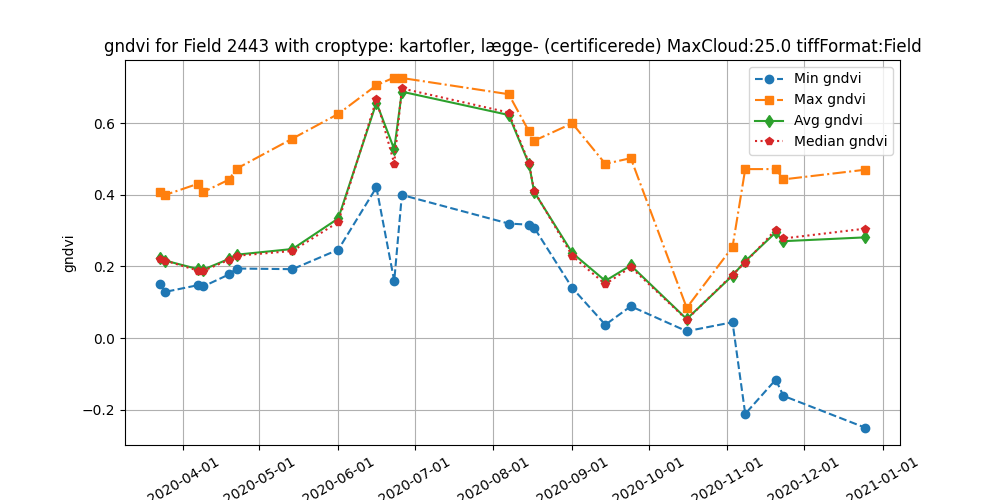
\includegraphics[width=\textwidth]{images/results/Field2443GNDVIGraph.png}
    \caption{GNDVI readings for Field ID 2443, seed potatoes (25\% max cloud coverage)}
    \label{fig:2443GNDVIavg}
  \end{minipage}
  \hfill
  \begin{minipage}[b]{0.42\textwidth}
    \centering
    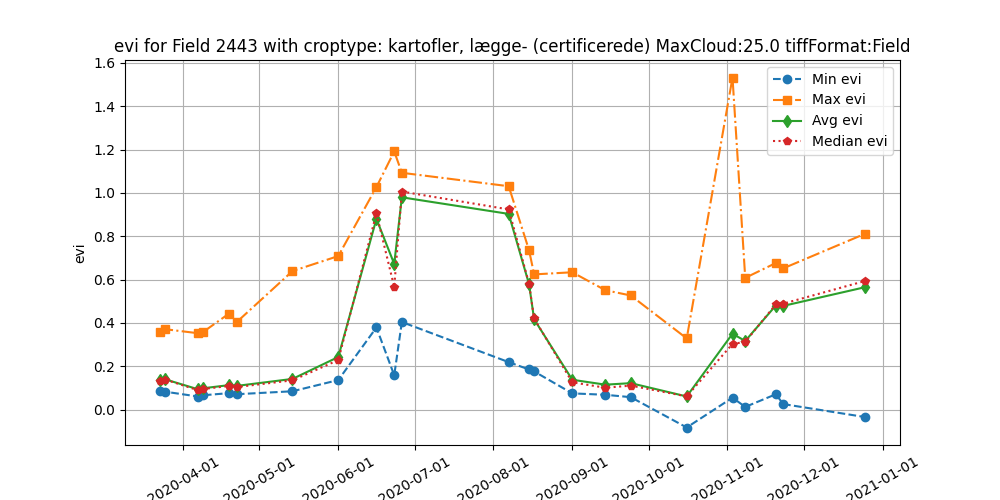
\includegraphics[width=\textwidth]{images/results/Field2443EVIGraph.png}
    \caption{EVI readings for Field ID 2443, seed potatoes (25\% max cloud coverage)}
    \label{fig:2443EVIavg}
  \end{minipage}
\end{figure}

EVI specializes in variability of crop development in relation to the leaf area index - bla bla ikke relevant index, videre
\textcolor{red}{EVI snak her - Skal have dobbelttjekket graf inden tho}

GNDVI does not saturate the same way NDVI does and generally has slightly lower values. But due to the green band focusing on green light reflectance off of chlorophyll, it is better at observing variance in chlorophyll levels across a vegetated area. \textcolor{red}{Mangler heatmaps her, har en teori om at der er større variance fra pixel til pixel med GNDVI? Krydser fingre}.

While GNDVI is more sensitive to variance in chlorophyll levels in plants and is most commonly used to detect stressed or aged vegetation in the intermediate to late growth stages. But similar to NDVI, its readings stem primarily from the canopy of the plant and the chlorophyll levels of the leaves, making it too similar in its usage.

\subsection{NDVI and NDRE readings}
Normalized Difference Red Edge Index is akin to GNDVI. It focuses of the chlorophyll levels of crops in the mid to late season, but differentiates itself by using the red edge spectrum, allowing it to "see" through the canopy, getting a fuller picture of the plants health. This has relevancy in multiple scenarios. Firstly, in the late season, if a crop is unaffected by pre-harvest crop desiccants and allowed its natural conclusion, the canopy will start to wilt. This will result in the NDVI values dropping, indicating stressed vegetation, which could be cause of alarm. But looking at an NDRE reading of the same crop, the readings might remain less affected as the vegetation beneath the canopy is still healthy\cite{eos_ndre}. In contrast, if the tuber or the stem of a crop becomes sick or lacks the proper nutrients, the canopy might still appear healthy. Here the NDVI values would remain high but a drop would be seen in the NDRE readings\cite{eos_ndre}.

Using NDVI and NDRE in combination is useful in determining the overall health of a crop, but it could also prove useful in determining the overuse of pre-harvest crop desiccants.

\begin{figure}[htbp]
    \centering
    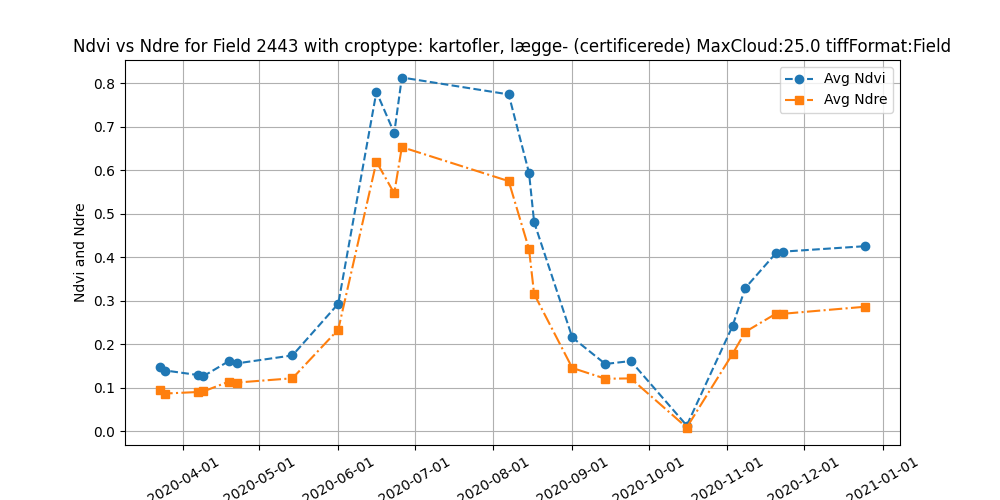
\includegraphics[width=0.75\linewidth]{images//results/Field2443NDREandNDVI.png}
    \caption{NDVI \& NDRE readings for Field ID 2443, seed potatoes (25\% max cloud coverage)}
    \label{fig:2443NDVIandNDREavg}
\end{figure}

Inspecting the same field using NDVI and NDRE on figure \ref{fig:2443NDVIandNDREavg}, it is expected to see NDRE follow along with NDVI throughout the growth cycle of the potato plant. It has a lower value than NDVI, which is expected, as the NDRE does not saturate like NDVI does and pierces to canopy to gets a clearer reading of the overall chlorophyll levels. Around August 7th where assumed pre-harvest crop desiccant application occurs, both indices drop significantly. Notably, the NDVI has a steeper decline over the desiccation period than the NDRE index. This could be because the crop desiccant is sprayed in liquid form and while it should kill both the leaves and the stem, it primarily hits the leaves, leading to a quicker wilting of the canopy and in turn steeper drop in NDVI values compared to NDRE values. This could also be why multiple applications of crop desiccants can be necessary. \textcolor{red}{Sidste assumption her skal jeg lige se om jeg kan undersøge og finde en kilde på}
Notably, both indices plateau at around 0,1 NDRE and 0,15 NDIin the middle of September, indicating the vegetation is dead and wilted. And both indices reach a value of near 0 on at harvest around October 16th.

\subsubsection{Heat maps}
\textcolor{red}{Faktisk lidt usikker på hvad jeg vil sige med heatmaps her? Måske bare lidt sådan "uha se der er varians", men idk. Virker lidt luftigt}

\subsection{Theoretical Pesticide Overuse Calculations} \label{Theoretical Pesticide Overuse Calculations}
Observed on figure \ref{fig:2443NDVIandNDREavg} the NDVI has a steeper decline compared to the NDRE index on August 7th, the assumed date of pre-harvest crop desiccant application. It is theorized that the causation for this is because the desiccant primarily hits the leaves, leading to a quicker wilting of the canopy and a faster decline in the NDVI. But should an overuse of pesticides be used, it is assumed that there would be a more thorough application to the entirety of the plant, including the stem, illustrated on figure \ref{fig:overuseIllustration}, which would lead to a steeper decline of the NDRE index.

\begin{figure}[htbp]
    \centering
    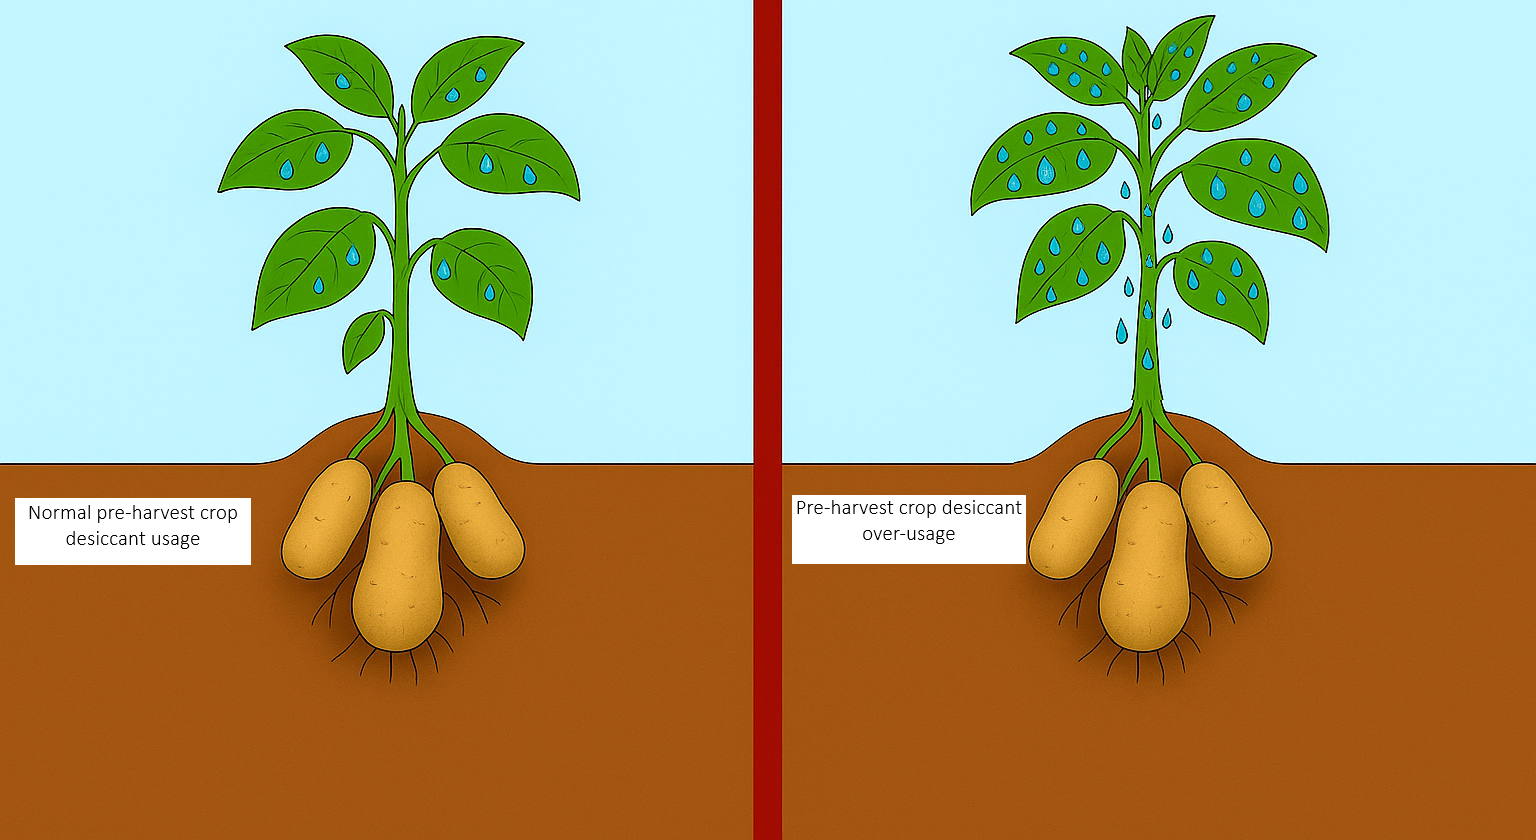
\includegraphics[width=0.75\linewidth]{images//results/potatovaffleri2.png}
    \caption{Theoretical Pre-harvest Desiccant Application and Overuse Application (generated from sketch using AI)}
    \label{fig:overuseIllustration}
\end{figure}

The following is a theoretical approach of finding trends that could be an indication of pre-harvest crop desiccant overuse. The approach is based of of NDVI being predominantly sensitive to leaf canopy degradation, while NDRE can penetrate deeper to asses overall biomass health and stress and how an overuse of desiccant agents would assumably affect the entirety of the plant more thoroughly, leading to a quicker decline of stem health along with the canopy.

On figure \ref{fig:Field2443Geogebra} the diagram has been plotted in GeoGebra and two linear lines have been drawn for NDVI and NDRE respectively. The pre crop desiccant use line (pre-line), is the best fitted linear line going through all of the points from the healthiest stage in June (highest chlorophyll levels) till the last point before the decline indicating crop desiccant use. And the post crop desiccant use line (post-line), which is the best fitted linear line going through all of the points from the start of the decline till the plateau.

\begin{figure}[htbp]
    \centering
    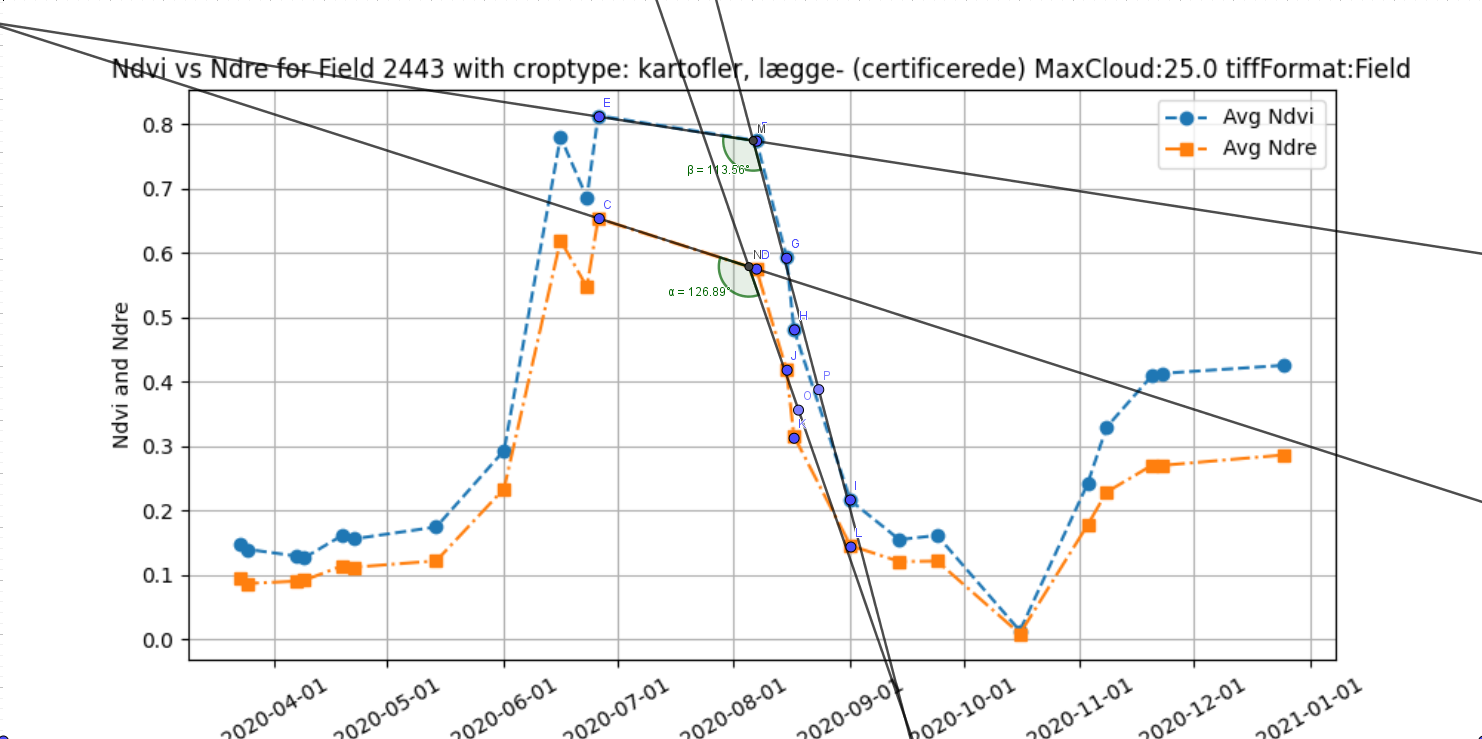
\includegraphics[width=0.75\linewidth]{images//results/Field2443Geogebra.png}
    \caption{Field 2443 angle analysis between pre- and post desiccant application linear decline}
    \label{fig:Field2443Geogebra}
\end{figure}

Measuring the angle between the pre-line and post-line for NDVI and NDRE, the NDRE angle should generally be broader compared to the NDVI angle, as the the NDVI post-line has a steeper decline. Comparing the two can be done by simple division of the two:

\begin{equation}
    \text{Overuse Score} = \frac{\text{NDVI-Angle}}{\text{NDRE-Angle}}
    \label{eq:overuse_score}
\end{equation}

This was done with a number of different fields growing seed potatoes in Denmark in the same year, where the graphs were plotted and the overuse score was calculated, as seen on table \ref{tab:field_overuse_scores}.

\begin{table}[htbp]
    \centering
    \begin{tabular}{cc}
        \hline
        \textbf{Field ID} & \textbf{Overuse Score} \\
        \hline
        2443 & 0,895 \\
        6079 & 0,887 \\
        8744 & 0,896 \\
        9530 & 1,07 \\
        9661 & 0,99 \\
        \hline
    \end{tabular}
    \caption{Field ID and Corresponding Overuse Scores}
    \label{tab:field_overuse_scores}
\end{table}

Using this logic, a clear trend emerges. The normal overuse scores lie around 0,9 and the closer they are to 1 or greater than 1, the greater the likelihood of desiccant overuse. An issue with this method is the lack of data due to cloud coverage. If the cloud coverage is greater than 25\% that days data point was excluded because of the extremity is noise levels. This presents the problem that some fields experienced long periods of cloudy days and lack data points. An example of this is seen on figure \ref{fig:Field9530Geogebra}

\begin{figure}[htbp]
    \centering
    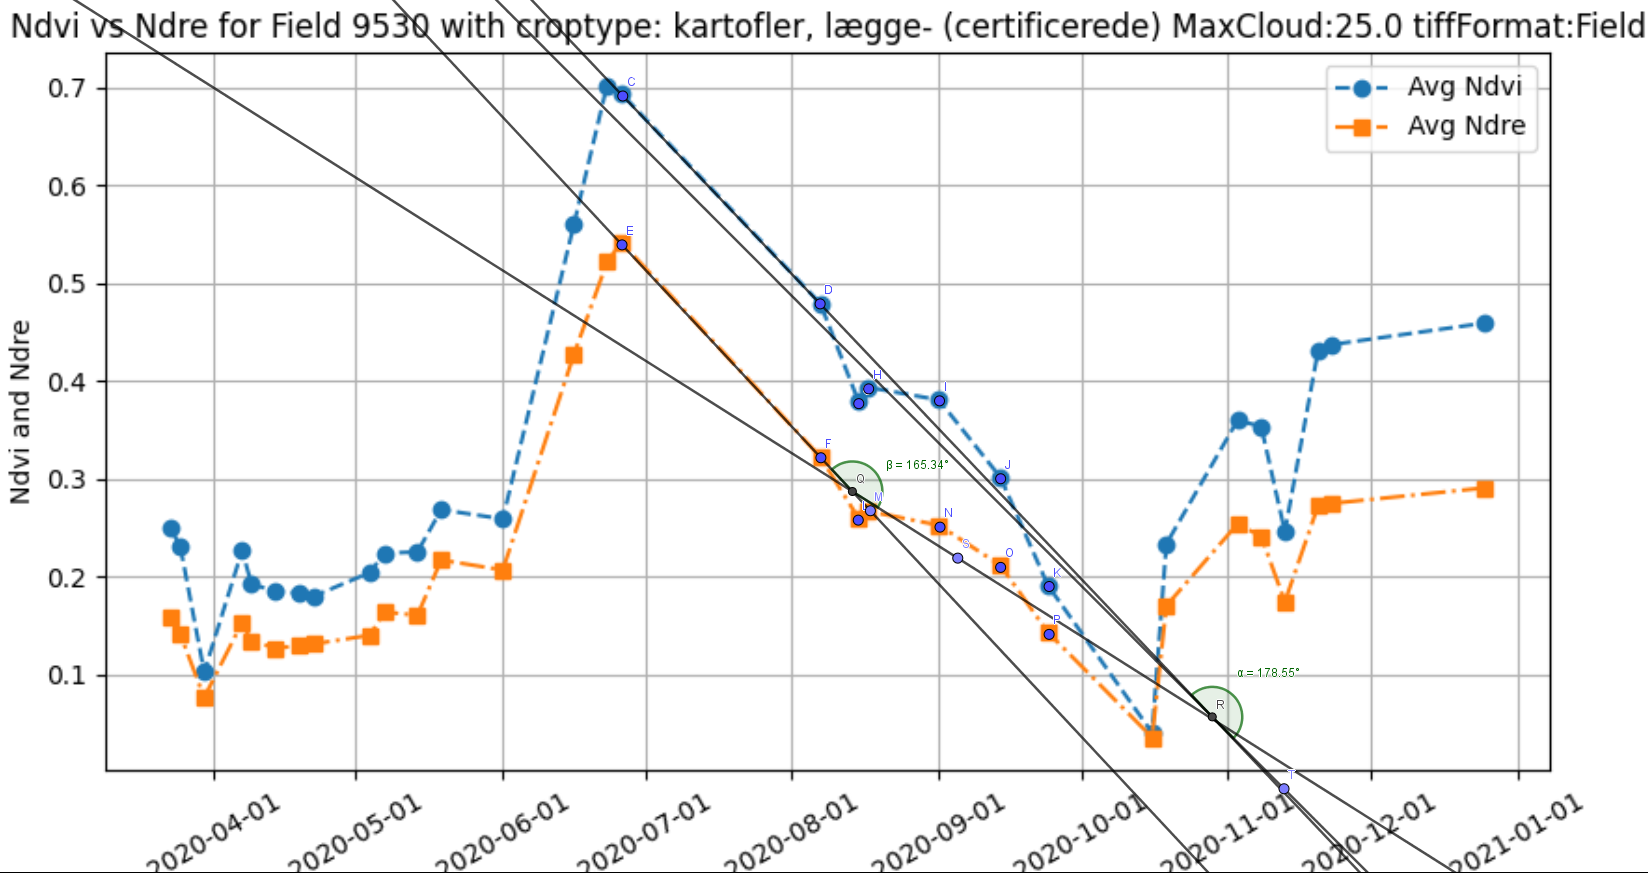
\includegraphics[width=0.75\linewidth]{images//results/Field9530Geogebra.png}
    \caption{Field 9530 angle analysis between pre- and post desiccant application linear decline}
    \label{fig:Field9530Geogebra}
\end{figure}